\documentclass[journal]{IEEEtran}

\usepackage{amsmath,amssymb}
\usepackage{graphicx}
\usepackage{xcolor}
\usepackage{mdframed}
\usepackage{booktabs}
\usepackage{hyperref}
\usepackage{tikz}
\usepackage{pgfplots}
\pgfplotsset{compat=1.18}
\usetikzlibrary{arrows.meta,positioning,shapes.geometric,fit,calc,backgrounds}

\definecolor{darkblue}{RGB}{0,0,139}
\definecolor{midgreen}{RGB}{34,139,34}
\definecolor{deepred}{RGB}{180,0,0}
\definecolor{steelblue}{RGB}{52,102,153}
\definecolor{tealcolor}{RGB}{0,110,110}
\definecolor{ambercolor}{RGB}{204,102,0}
\definecolor{slateblue}{RGB}{90,80,160}

\hypersetup{colorlinks=true,linkcolor=darkblue,citecolor=darkblue,urlcolor=darkblue}

\makeatletter
\def\abstract{\normalfont
    \if@twocolumn
      \relax
    \else
      \bgroup\par\addvspace{0.5\baselineskip}\centering\vspace{-1.78ex}%
      \@IEEEabskeysecsize\textbf{\abstractname}%
      \par\addvspace{0.5\baselineskip}\egroup\quotation\@IEEEabskeysecsize
    \fi\@IEEEgobbleleadPARNLSP}
\def\IEEEkeywords{\normalfont
    \if@twocolumn
      \relax
    \else
      \bgroup\par\addvspace{0.5\baselineskip}\centering\@IEEEabskeysecsize%
      \textbf{\IEEEkeywordsname}%
      \par\addvspace{0.5\baselineskip}\egroup\quotation\@IEEEabskeysecsize
    \fi\@IEEEgobbleleadPARNLSP}
\makeatother

\begin{document}

\title{\textcolor{darkblue}{Could Artificial Intelligence Be Replaced With
Biocomputing Intelligence?}}

\author{\IEEEauthorblockN{\textcolor{slateblue}{\itshape Muhammad Faisal Laiq \qquad
Email:~shmlaiq@gmail.com \qquad ORCID:~0009-0007-5779-9836}}}

\maketitle

\begin{abstract}
\begin{mdframed}[
  linecolor=darkblue, linewidth=1.8pt,
  backgroundcolor=darkblue!5,
  innerleftmargin=10pt, innerrightmargin=10pt,
  innertopmargin=9pt, innerbottommargin=9pt,
  roundcorner=5pt, skipabove=0pt, skipbelow=0pt
]
\noindent\textbf{\textcolor{darkblue}{Abstract\,---}}~Biocomputing systems built from
living neurons---most visibly Cortical Labs' DishBrain and CL1, which taught cultured
neurons to play Pong and, more recently, Doom---are increasingly framed as a
resource-driven successor to conventional silicon AI. This paper evaluates that claim
against three necessary conditions: capability parity, resource superiority at
data-center scale, and the absence of a disqualifying hidden cost, mapping three
existing systems onto the evaluation. On capability, biocomputing systems show real,
measured learning, but independent testing on one system found most of the apparent
intelligence traced to conventional silicon scaffolding, not the biological
substrate---parity is partial and unverified at the substrate level. On resource
superiority, the efficiency case is real per neuron but has no demonstrated path to
scale: without a vascular system, cultured tissue cannot sustain a viable core beyond
roughly 475 micrometers in radius, orders of magnitude below data-center scale, and no
system has published a solution. On hidden cost, capability and moral-status risk are
logically independent properties, not two ends of one dial---shown directly by a 2022
paper's use of ``sentience'' for a capability finding and the 30-scientist rebuttal it
triggered---so every efficiency gain biocomputing offers is bought with a risk
category silicon AI does not carry. The honest current answer is no, ordered by which
gap is most urgent to close: not because the biology is uninteresting, but because
condition two fails on a specific, peer-reviewed physical constraint funding and
algorithms cannot resolve, and condition three imposes a cost no public comparison
currently prices.
\end{mdframed}
\end{abstract}

\begin{IEEEkeywords}
\begin{mdframed}[
  linecolor=darkblue, linewidth=0.8pt,
  backgroundcolor=darkblue!3,
  innerleftmargin=8pt, innerrightmargin=8pt,
  innertopmargin=6pt, innerbottommargin=6pt,
  roundcorner=4pt, skipabove=4pt, skipbelow=0pt
]
\noindent\textbf{\textcolor{darkblue}{Index Terms}}\,---~biocomputing, organoid
intelligence, artificial intelligence comparison, moral status, consciousness
science, risk stratification
\end{mdframed}
\end{IEEEkeywords}

\section{\textcolor{darkblue}{Introduction}}

In March 2025, Cortical Labs began shipping a $\$35{,}000$ desktop unit built around
living human neurons \cite{corticallabs2025cl1}. The unit, called CL1, is a commercial
descendant of DishBrain, a 2022 research prototype in which roughly 800{,}000 cultured
neurons learned to play Pong within minutes of real-time gameplay
\cite{kagan2022dishbrain}. In 2026, an independent collaborator used Cortical Labs'
own API to get a CL1 unit playing Doom---a substantially harder, non-linear,
exploration-requiring task---in under a week, a detail the company narrates directly
in its own product demonstration \cite{corticallabs2026doom}. Both results have been
covered widely in general and technology media, in registers ranging from
straightforward technical explanation \cite{bloomberg2025biocomputing} to explicit
alarm about whether the technology raises questions society is not equipped to answer
\cite{notready2026biocomputing}, and a consistent thread runs through nearly all of
that coverage: biocomputing is framed as a response to conventional AI's resource
crisis, a biological substrate that could someday replace silicon because it learns
from less data on a fraction of the power. None of that popular coverage is treated
in this paper as scientific evidence; we cite it only because it accurately reflects
the terms in which this technology is actually being discussed outside the
laboratory---and because that framing deserves a direct, falsifiable answer rather
than a vague sense that the technology ``could eventually'' scale.

This paper supplies that answer by decomposing the replacement claim into three
conditions that all have to hold simultaneously, not just individually plausible in
isolation. \emph{Capability parity} asks whether the biological substrate itself,
not surrounding conventional hardware, is doing the learning. \emph{Resource
superiority at scale} asks whether the efficiency case that motivates the whole
comparison actually has a demonstrated path from a single cultured dish to
anything resembling data-center throughput. \emph{No disqualifying cost} asks
whether pursuing that efficiency case is free of a cost silicon AI does not carry at
all. A ``yes'' to the paper's title question requires all three. This paper finds one
holds only partially, one fails on a specific physical constraint, and one fails by
construction---and argues that finding is more useful than an aggregate verdict, because
each condition points to a different, independently addressable research gap.

The capability question has a precise and instructive origin. When Kagan et al.
published the DishBrain result, they described the neuron culture as exhibiting
``sentience''---defined in the paper in a narrow, functional sense: responsiveness to
sensory input in a goal-directed way \cite{kagan2022dishbrain}. Thirty neuroscientists
signed a published rebuttal whose primary and most developed concern was exactly that
terminology: that ``sentience,'' ``intelligence,'' and ``goal-directed behavior'' were
being applied to cultured neurons without the conceptual grounding those terms carry
elsewhere in neuroscience and bioethics, and that this risked misleading both
scientific peers and the public about what the result actually showed---including,
the signatories noted, creating a downstream financial incentive to keep using
inflated language for the methods described \cite{balci2023response}. But the
rebuttal was not purely terminological: it also stated directly that some of the
study's conclusions were compromised by results that failed to adequately match
control and experimental conditions---a methodological objection that brushes
against the capability claim itself, not only its label. Kagan et al.'s own published
reply concedes the terminology critique is worth taking seriously while defending
their operational definition as principled rather than promotional, and does not
substantively rebut the control-condition concern \cite{kagan2023reply}. This paper
treats that dispute as the first documented instance of exactly the pattern a
replacement claim risks repeating at larger scale: a capability finding gets
described in language that implies more than the data supports, and the field has
not adopted a vocabulary that would prevent the same overreach from happening again
with the next milestone---including, this paper argues, the milestone of ``ready to
replace conventional AI.''

The contributions of this paper are as follows:
\begin{itemize}
\item We decompose the AI-replacement claim into three explicit, individually
testable necessary conditions---capability parity, resource superiority at scale,
and no disqualifying cost---rather than evaluating it as one aggregate question, so
that each finding points to a specific, addressable gap rather than a diffuse verdict.
\item On resource superiority, we identify a concrete bioengineering limit---the
diffusion-limited size ceiling on unvascularized biological
tissue---that caps viable biocomputing substrate far below what data-center-scale
deployment would require, and that no biocomputing system studied here has
published a solution to it.
\item On disqualifying cost, we give a construction argument, not an empirical one,
for why a biocomputing system's demonstrated capability and its moral-status risk can
vary on separate axes entirely rather than trading off along one---a claim
that does not require solving the hard problem of consciousness to be useful, only
requiring that capability and risk not be conflated in language or governance.
\item We map three existing systems---DishBrain, CL1, and FinalSpark's
Neuroplatform---against all three conditions, and compare biocomputing to
conventional silicon AI across the specific dimensions the conditions require:
energy efficiency, data efficiency, scale trajectory, and the risk dimension that
comparison usually omits entirely.
\end{itemize}

The remainder of this paper proceeds as follows. Section~II reviews three
literatures this paper draws on: biocomputing and organoid intelligence,
consciousness science, and AI capability evaluation. Section~III traces the
technical lineage from DishBrain to CL1 and the training mechanism both rely on.
Section~IV evaluates the three necessary conditions in turn, including the
capability/risk framework and its theoretical grounding. Section~V maps three
systems onto that evaluation. Section~VI states limitations directly. Section~VII
concludes with a direct answer and a research agenda ordered by urgency.

\section{\textcolor{darkblue}{Related Work}}

\subsection{\textcolor{steelblue}{Biocomputing and Organoid Intelligence}}

The technical foundation for growing neurons that were never part of a living brain
traces to Yamanaka's reprogramming work: four defined transcription
factors---Oct3/4, Sox2, Klf4, and c-Myc---can reset a mature skin cell back to a
pluripotent state from which it can be redirected into almost any cell type,
including a neuron \cite{takahashi2006induction}. The human-cell version of this
result, published a year later, meant researchers no longer needed neural tissue
extracted from a living or donated brain; a small skin sample was sufficient
\cite{takahashi2007induction}. Every biocomputing system discussed in this paper
depends on this result, directly or through cultures descended from it. Kagan et
al.'s DishBrain assembled roughly 800{,}000 such neurons on a high-density
multielectrode array, embedded the culture in a closed-loop simulated Pong
game-world, and reported a statistically significant increase in successful paddle
returns within five minutes of gameplay---the paper's operational definition of
learning \cite{kagan2022dishbrain}. A large multi-author position paper coined the
term ``organoid intelligence'' for the broader research program this result opened,
arguing that three-dimensional neural organoids---rather than flat cultures---could
eventually support far more complex computation, and grounding the case for pursuing
this on efficiency terms: an estimated $10^{6}$-fold power advantage over a
comparable digital system on certain classes of problem, and comparable data
efficiency claims relative to conventional machine learning \cite{smirnova2023organoid}.
FinalSpark's Neuroplatform operationalizes a related but distinct model: sixteen
brain organoids, roughly 160{,}000 total neurons, made remotely accessible online for
a monthly access fee, described in a peer-reviewed system paper that documents the
platform's architecture without making the more dramatic efficiency claims that have
since circulated in press coverage about the company \cite{jordan2024open}. None of
this literature evaluates the replacement question against explicit necessary
conditions; each paper argues its own system is a promising step, not that biocomputing
as a category currently satisfies what replacing conventional AI would require. That
is the gap this paper works to fill.

\subsection{\textcolor{tealcolor}{Consciousness Science and Moral Status}}

Chalmers' original statement of the hard problem draws the distinction Section~IV's
third condition depends on: explaining a system's functional, behavioral capacities
is one problem, and explaining why any of that functioning is accompanied by
subjective experience at all is a separate, harder problem that functional
explanation does not automatically resolve \cite{chalmers1995facing}. Solms argues
for a specific, falsifiable-in-principle position on where experience originates:
not as a property that emerges once cognition becomes sufficiently sophisticated, but
as more evolutionarily basic than cognition, arising from homeostatic,
affect-regulating circuitry that predates cortex \cite{solms2019hard}. This matters
directly for biocomputing, because the free-energy-principle training method every
system in this paper's case mapping uses---rewarding a culture with predictable
stimulation when it succeeds and punishing it with chaotic, unpredictable
stimulation when it fails---is architecturally a version of exactly the
predict-and-minimize-surprise loop Solms locates as affect's origin
\cite{kagan2022dishbrain}. If Solms is right, that training method is not incidental
to the cost question this paper's third condition asks about; it is that question,
applied as an engineering technique rather than examined as one. Independently of
any theory of where experience originates, there is direct empirical evidence that
humans are poor at detecting its presence even in other humans. Owen et al. found
that a patient who met every clinical criterion for a vegetative diagnosis showed
fMRI activation, on request to imagine playing tennis, indistinguishable from healthy
volunteers performing the same task---evidence of covert awareness a bedside
behavioral exam had missed entirely \cite{owen2006detecting}. Two independent
follow-up studies converge on this not being a rare exception: Monti et al. found
four of twenty-three behaviorally vegetative patients could willfully modulate their
own brain activity on command \cite{monti2010willful}, and a larger, more recent
multi-site study found evidence of this covert cognitive-motor dissociation in
approximately one quarter of clinically unresponsive patients
\cite{bodien2024cognitive}, while a systematic review using more conservative
criteria places the figure closer to fifteen percent \cite{kondziella2016systematic}.
The exact rate is contested; the direction of the finding is not. If clinicians with
a fully human patient in front of them, using validated diagnostic criteria, miss
covert awareness in roughly one in six to one in four cases, the base rate for
correctly assessing whatever is or is not present in a dish of neurons should be
assumed worse, not better, absent a specific reason to think otherwise.

\subsection{\textcolor{ambercolor}{AI Capability Evaluation}}

A separate, purely computational literature establishes the terms this paper's
resource-superiority condition needs. Patterson et al. measured GPT-3's training
energy consumption directly at 1{,}287 megawatt-hours, with total carbon footprint
varying by up to a factor of fifty depending on the training data center's local
grid composition \cite{patterson2021carbon}---a precise, audited figure this paper
prefers over the rounder, less-sourced estimates that circulate in secondary
biocomputing literature. Epoch AI's continuously updated compute-trend analysis
finds that training compute for notable AI models has grown roughly 4.4-fold per
year since 2010, a pace that has further accelerated for frontier models released
since 2020, with the most recent releases showing doubling times as short as three
to four months \cite{epoch2025compute}. Neither of these sources is biocomputing
literature; we use them because a fair replacement evaluation requires a real,
audited baseline for what conventional AI actually costs, not a figure borrowed
secondhand from a biocomputing paper's own citation of it. Underlying both the
biocomputing efficiency claims and the consciousness-science affect argument is a
basic physiological fact: the human brain, at roughly two percent of body mass,
consumes approximately twenty percent of resting metabolic energy, translating to an
estimated twenty watts of continuous power draw \cite{raichle2002appraising,
attwell2001energy}. This number appears, uncredited to its physiological source, in
nearly every popular account of biocomputing's efficiency case; we cite the primary
neuroscience literature directly rather than repeat it as an unattributed round
number.

\section{\textcolor{darkblue}{Background: From DishBrain to CL1}}

Both systems this paper treats as primary cases share one training mechanism,
first demonstrated at scale by DishBrain and carried forward, apparently unchanged
in its basic logic, into CL1. A living neuron culture sits on a multielectrode
array divided into sensory and motor regions. A game engine translates its internal
state---ball position in Pong, an approaching enemy in Doom---into an electrical
stimulation pattern delivered to the sensory region. The culture's spontaneous and
evoked firing in the motor region is read back out and mapped to an action: paddle up
or down; move, turn, or shoot. Neither game engine grants the culture any innate
knowledge of what it is controlling. The behavioral shaping happens entirely through
consequence: a missed action is followed by unpredictable, high-entropy stimulation
across the array, and a successful action is followed by calm, predictable
stimulation \cite{kagan2022dishbrain}. Kagan and colleagues explain this design
choice by appeal to the free energy principle---the proposition that living systems
generally act so as to minimize surprise, because an organism that cannot predict the
consequences of its own actions cannot reliably keep itself alive. Under that
account, the culture is not learning to win a game in any sense that requires
understanding what a game is; it is minimizing an aversive signal, and winning the
game is the observable side effect.

Cortical Labs' own account of moving this mechanism from Pong to Doom is instructive
about what, specifically, improved between 2022 and 2026---and it is the paper's
first evidence relevant to the capability-parity condition. Pong offers a single,
direct input-output relationship---ball position maps to one correct paddle
direction---and took the company's original hardware and software over eighteen
months to get working reliably. Doom is qualitatively harder: three-dimensional,
populated with enemies in varying positions, requiring the system to explore an
environment rather than track one variable. Using a matured software interface the
company calls its API, running on a cloud platform it calls Cortical Cloud, an
independent collaborator implemented the Doom mapping---enemy position to
directional stimulation, spike pattern to shoot-or-turn-or-move command---in under a
week \cite{corticallabs2026doom}. The company is explicit in its own account that the
resulting player is not skilled: it dies constantly, plays, in the presenting
scientist's own phrase, ``like a beginner who's never seen a computer,'' but shows
consistent goal-seeking behavior---locating and firing at enemies---that counts as
evidence of ongoing learning \cite{corticallabs2026doom}. What changed across four
years was the interface and the encoding scheme, not the underlying biological
mechanism, which is the same predict-and-minimize-surprise loop DishBrain used. As
Section~IV-A discusses, that distinction matters directly for capability parity: an
improved interface is evidence the surrounding engineering matured, not by itself
evidence the biological substrate's own contribution grew at the same rate.

\begin{figure}[!t]
\centering
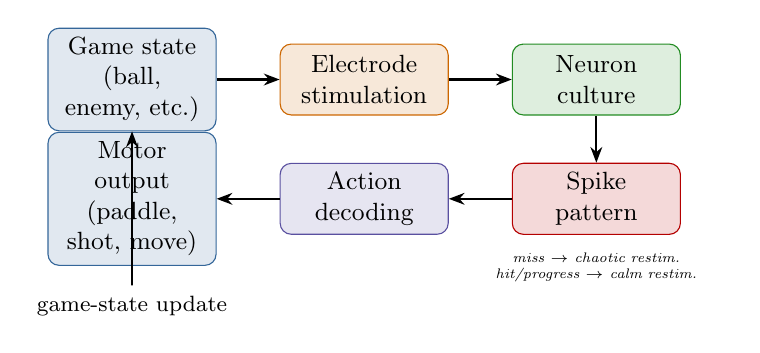
\begin{tikzpicture}[
  node distance=6mm and 8mm,
  box/.style={draw, rounded corners, align=center, minimum height=9mm,
    text width=19mm, font=\small},
  arr/.style={-{Stealth[length=2mm]}, thick}
]
\node[box, fill=steelblue!15, draw=steelblue] (game) {Game state\\(ball, enemy, etc.)};
\node[box, fill=ambercolor!15, draw=ambercolor, right=of game] (stim) {Electrode\\stimulation};
\node[box, fill=midgreen!15, draw=midgreen, right=of stim] (cult) {Neuron\\culture};
\node[box, fill=deepred!15, draw=deepred, below=of cult] (spike) {Spike\\pattern};
\node[box, fill=slateblue!15, draw=slateblue, left=of spike] (decode) {Action\\decoding};
\node[box, fill=steelblue!15, draw=steelblue, left=of decode] (act) {Motor output\\(paddle, shot, move)};
\draw[arr] (game) -- (stim);
\draw[arr] (stim) -- (cult);
\draw[arr] (cult) -- (spike);
\draw[arr] (spike) -- (decode);
\draw[arr] (decode) -- (act);
\draw[arr] (act) -- ++(0,-11mm) -| (game)
  node[midway, below, font=\footnotesize] {game-state update};
\node[below=1mm of spike, font=\tiny\itshape, text width=32mm, align=center]
  {miss $\to$ chaotic restim.\\hit/progress $\to$ calm restim.};
\end{tikzpicture}
\caption{The closed-loop training mechanism shared by DishBrain and CL1: game
state is encoded as electrode stimulation, the neuron culture's spiking response
is decoded into a motor action, and the resulting outcome determines whether the
next stimulation is calm/predictable (success) or chaotic/unpredictable (failure)
\cite{kagan2022dishbrain, corticallabs2026doom}.}
\label{fig:loop}
\end{figure}

Fig.~\ref{fig:loop} depicts this shared mechanism. One inconsistency is worth naming
directly rather than silently resolving, because it illustrates the precision problem
this paper argues the field has more broadly whenever a capability or scale claim is
made. Cortical Labs' own launch-period press materials and independent technology
coverage consistently describe CL1 as containing approximately 800{,}000 neurons, the
same order of magnitude as the original DishBrain prototype \cite{corticallabs2025cl1}.
Cortical Labs' own Doom demonstration video, by contrast, states the specific unit
shown contains ``around 200{,}000'' neurons \cite{corticallabs2026doom}. Both
statements come from the company itself; we could not find a reconciliation of the
two figures in any source consulted for this paper, and we decline to silently pick
one. Readers should treat CL1's neuron count as company-stated but internally
inconsistent across the company's own communications, not as a settled specification.

\section{\textcolor{darkblue}{Three Conditions for Replacement}}

A ``yes'' answer to this paper's title question requires all three of the following
conditions to hold at once. Each is evaluated in turn.

\subsection{\textcolor{slateblue}{Condition 1: Capability Parity}}

Capability parity asks whether the biological substrate itself, not surrounding
conventional hardware, is doing the learning a biocomputing system exhibits. We
assess it, $C \in [0,1]$, against four criteria: (i) whether the system demonstrates
statistically significant, above-chance improvement on a closed-loop task; (ii)
sample efficiency, i.e.\ how much interaction is required before that improvement
appears; (iii) generalization, whether performance transfers to a task variant the
system was not directly trained on; and (iv) the proportion of the pipeline's
decision-making that is attributable to conventional computational scaffolding
around the biological substrate, rather than to the substrate itself.

Criterion (iv) is the condition's decisive one, and the evidence for it is
uncomfortable for a straightforward ``yes.'' Independent commentary on the CL1 Doom
demonstration reports a specific test: the system's developer, on suspecting a
conventional AI component might be doing most of the work, replaced the neuron
culture with pure random noise and found that learning stopped entirely
\cite{notready2026biocomputing}---indicating the culture was contributing something
real, but that a conventional AI component was doing most of the surrounding decision
work regardless. This is not grounded in a peer-reviewed source in this paper---the
test is reported only in independent commentary on the demonstration, not in a
company technical publication or peer-reviewed study, and we were unable to locate
either---but it is a design-relevant caveat any capability score for these systems
should carry, since it directly affects how much of an apparent capability advance is
properly attributed to the biological component at all rather than to the silicon
scaffolding this paper's title question is asking whether biology can replace.
Verdict: capability parity is real but partial, and currently unverified at the
substrate level for any system in this paper's case mapping.

\subsection{\textcolor{ambercolor}{Condition 2: Resource Superiority at Scale}}

Resource superiority at scale asks whether the efficiency case that motivates the
whole replacement comparison actually has a demonstrated path from a single cultured
dish to anything resembling data-center throughput. Table~\ref{tab:comparison}
compares biocomputing against conventional silicon AI across the dimensions this
condition requires.

\begin{table}[!t]
\centering
\caption{Biocomputing versus conventional silicon AI. Efficiency figures are the
most defensible, primary-sourced values found during this paper's literature
verification; several widely circulated figures (10~GWh for GPT-3 training; ``a
million times'' power advantage for organoid platforms) are marked as unverified
because they could not be traced to a peer-reviewed primary source at time of
writing.}
\label{tab:comparison}
\begin{tabular}{@{}p{2.1cm}p{2.5cm}p{2.9cm}@{}}
\toprule
\textbf{Dimension} & \textbf{Conventional AI} & \textbf{Biocomputing} \\
\midrule
Substrate & Silicon transistors (GPU/CPU/TPU dies) & Cultured human neurons on
electrode arrays or in organoid form \cite{kagan2022dishbrain, jordan2024open} \\
Hardware state & Fixed architecture once fabricated; weights updated, circuit
topology does not & Structurally plastic: connections between living neurons can
physically reorganize during training, not only weighted \cite{kagan2022dishbrain} \\
Training energy (reference case) & 1{,}287~MWh, GPT-3 \cite{patterson2021carbon} &
No comparably audited training-energy figure located; brain-scale estimate is
$\sim$20~W continuous \cite{raichle2002appraising}. A full commercial CL1 rack,
including life support, draws a company-communicated
$\sim$850--1{,}000~W operating (not training) power---a launch-coverage figure,
not a peer-reviewed one \cite{thompson2025cl1launch} \\
Compute/scale growth & $\sim$4.4$\times$/yr since 2010; 3--6~month doubling for
frontier models \cite{epoch2025compute} & No comparable trend data published; single
generations (Pong$\to$Doom) improved over $\sim$4~years \cite{corticallabs2026doom} \\
Learning mechanism & Gradient descent over a fixed, differentiable objective &
Predict-and-minimize-surprise stimulus/response shaping, not backpropagation
\cite{kagan2022dishbrain} \\
Maturity & Multi-decade, standardized tooling & Single-digit years; two companies
with materially different architectures \cite{jordan2024open} \\
Moral-status risk (Condition 3) & Effectively zero under current consciousness
science & Nonzero and currently unmeasurable (Section~IV-C) \\
\bottomrule
\end{tabular}
\end{table}

The per-neuron efficiency case in Table~\ref{tab:comparison} is real: brain-scale
power draw against data-center-scale power draw, and human sample efficiency against
machine sample efficiency, both favor biocomputing by a wide margin at the scale
measured so far. But condition 2 asks about scale, not per-unit efficiency, and that
is where the case runs into a concrete physical limit established in the
peer-reviewed organoid literature---one no amount of funding or algorithmic
cleverness touches. Without a vascular system to actively
deliver oxygen and nutrients, living tissue can sustain viable cells only within a
few hundred micrometers of its surface, because diffusion alone cannot supply an
actively metabolizing core beyond that distance. Allometric modeling of organoid
viability places the size ceiling at approximately 475 micrometers in radius for a
gel-encased structure before a hypoxic, non-viable core begins to form
\cite{magliaro2019allometric}---a scale several orders of magnitude below anything
resembling a data-center-scale processing unit. A biological brain avoids this limit
through a dense capillary network that actively perfuses tissue rather than relying
on passive diffusion; no biocomputing system studied in this paper, and none
identified in the wider literature at time of writing, has demonstrated a comparable
vascularization solution at any scale larger than a single small organoid. This is
not a claim that biocomputing's efficiency advantage is fake---the per-neuron energy
figures in Table~\ref{tab:comparison} are real and independently sourced---it is a
claim that the advantage does not currently have a demonstrated path to the scale at
which it would need to operate to functionally replace, rather than supplement,
conventional AI infrastructure. Claims to the contrary that circulate in press
coverage---the ``million times less power'' figure this paper already flags as
untraceable to any peer-reviewed FinalSpark publication, and larger, still
less-sourced multipliers that appear in secondary technology-press aggregation
rather than in any company or scientific publication this paper could
verify---should be read against this unresolved scaling constraint, not
independently of it. The only system-level operating-power figure located for a
complete commercial unit---the $\sim$850--1{,}000~W drawn by a full CL1 rack,
life-support subsystem included \cite{thompson2025cl1launch}---cuts the other way
from the ``million times less'' framing: it is a real device drawing power in the
same order of magnitude as a single high-end GPU, not a negligible fraction of one,
once the non-neural infrastructure a cultured-neuron system actually requires to
stay alive is counted rather than quietly excluded.

\begin{mdframed}[
  linecolor=ambercolor, linewidth=1.4pt,
  backgroundcolor=ambercolor!5,
  innerleftmargin=8pt, innerrightmargin=8pt,
  innertopmargin=6pt, innerbottommargin=6pt,
  roundcorner=4pt
]
\noindent\textbf{\textcolor{ambercolor}{Key Finding ---}}~Biocomputing's efficiency
advantage is real per neuron but has no demonstrated path past a $\sim$475-micrometer
diffusion-limited size ceiling---nowhere near the scale data-center deployment would
require---making condition 2 the clearest of the three conditions to fail, and the
one least likely to be resolved by funding or algorithmic progress alone.
\end{mdframed}

Verdict: resource superiority at scale fails, not on economic or algorithmic
grounds, but on an unsolved bioengineering constraint---vascularizing cultured
neural tissue---that no system in this paper's case mapping has published a
solution to.

\subsection{\textcolor{deepred}{Condition 3: No Disqualifying Cost}}

Even where conditions 1 and 2 might eventually be satisfied, a genuine replacement
claim requires that pursuing it carry no cost conventional silicon AI is exempt
from. This paper argues biocomputing fails this condition by construction, because
capability and moral-status risk move along separate axes entirely---pushing one
upward does nothing to the other, in either direction.

We define moral-status risk, $R \in [0,1]$, deliberately \emph{not} as an estimated
probability of consciousness; no instrument exists that could produce such an
estimate, and this paper does not claim otherwise. Instead we define $R$ as an
enumerable checklist score across five substrate properties that current
consciousness science treats as relevant, whether or not any of them is individually
sufficient: (i) living versus non-living tissue; (ii) presence of a homeostatic,
predict-and-minimize-surprise feedback loop of the kind Solms associates with the
origin of affect \cite{solms2019hard}; (iii) structural organization, with a flat
two-dimensional culture scoring lower than a three-dimensional organoid with
self-organized layered structure; (iv) human, as opposed to non-human animal or
fully synthetic, cellular provenance; and (v) absence of a validated test capable of
ruling experience out, which we include as a criterion in its own right because
Owen et al.'s finding demonstrates that absence of behavioral evidence is not
evidence of absence \cite{owen2006detecting}.

The claim that $C$ and $R$ are independent, not two ends of a single dial, is a
design argument, not an empirical one, and it can be shown by construction rather
than by appeal to any single system's measured values.

\emph{Claim.} There exist, or could straightforwardly exist, systems $s_1, s_2$ such
that $C(s_1) < C(s_2)$ while $R(s_1) = R(s_2)$, and systems $s_3, s_4$ such that
$R(s_3) < R(s_4)$ while $C(s_3) = C(s_4)$.

\emph{Argument for the first pair.} DishBrain and CL1 running its early Pong-only
configuration versus CL1 running its matured Doom configuration satisfy this
directly. Section~III establishes that the interface and encoding scheme improved
substantially between the two---longer training time and a simpler task in one case,
a harder task solved faster with a matured API in the other---which is precisely what
criterion (ii) and (iii) of $C$ are built to register as a difference. None of
$R$'s five criteria changed: both are living, human-derived, cultured on a flat
electrode array, trained with the same predict-and-minimize-surprise loop, and
neither can be ruled out or in on experience by any existing test. A capability
advance occurred with the risk profile held fixed.

\emph{Argument for the second pair.} Consider a flat two-dimensional neuron culture
that has not yet been embodied in any closed-loop task at all---$C \approx 0$ by
criterion (i), since no learning has been demonstrated---against a fully-formed,
three-dimensionally organized organoid that has likewise not been embodied in any
task. Both score $C \approx 0$. But the organoid scores higher on $R$ purely by
virtue of criterion (iii)'s structural-organization term: a self-organized,
layered, three-dimensional structure is closer to features consciousness science
treats as potentially relevant than an unstructured flat sheet is, independent of
whether either has ever been asked to do anything. Risk, on this account, can be
present before capability is demonstrated at all, which is exactly why treating an
untrained system as risk-free because it has not yet ``done anything impressive'' is
a category error, not merely an overcautious position.

\begin{mdframed}[
  linecolor=deepred, linewidth=1.4pt,
  backgroundcolor=deepred!5,
  innerleftmargin=8pt, innerrightmargin=8pt,
  innertopmargin=6pt, innerbottommargin=6pt,
  roundcorner=4pt
]
\noindent\textbf{\textcolor{deepred}{Key Finding ---}}~Capability and moral-status
risk can move independently in both directions: a capability jump can occur with
risk held fixed (DishBrain to CL1-Doom), and risk can be nonzero before any
capability is demonstrated at all (an untrained three-dimensional organoid). Every
efficiency gain condition 2 might eventually deliver is therefore bought with a risk
category conventional silicon AI is exempt from entirely---the disqualifying cost
condition 3 asks about.
\end{mdframed}

A corollary follows directly: because $R$ can be nonzero at $C \approx 0$, a
governance or reporting policy that gates ethical scrutiny on capability
milestones---review it once it does something impressive---is misaligned with what
the checklist criteria above actually track. The living-tissue and human-provenance
criteria are present at the moment cells are cultured, not at the moment a
demonstration succeeds. Verdict: condition 3 fails by construction, independent of
how conditions 1 and 2 eventually resolve.

\section{\textcolor{darkblue}{Case Mapping}}

\begin{figure}[!t]
\centering
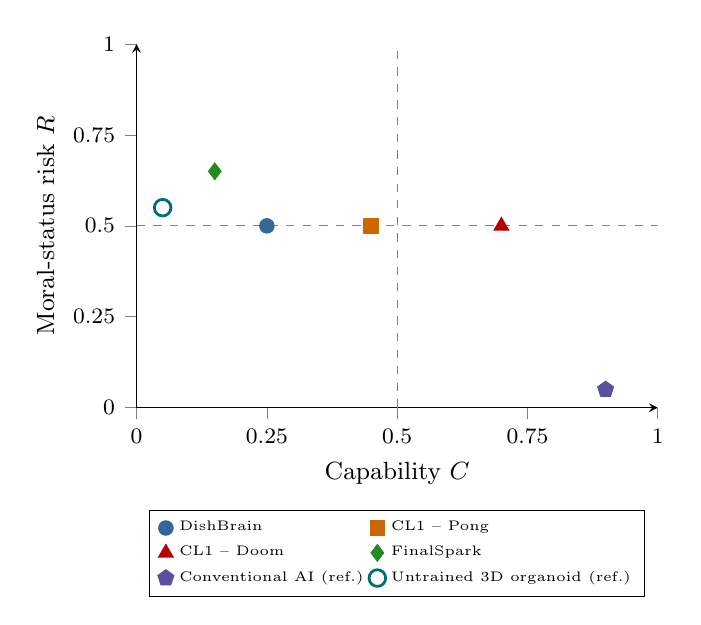
\begin{tikzpicture}
\begin{axis}[
  width=8.2cm, height=6.2cm,
  xlabel={Capability $C$}, ylabel={Moral-status risk $R$},
  xmin=0, xmax=1, ymin=0, ymax=1,
  xtick={0,0.25,0.5,0.75,1}, ytick={0,0.25,0.5,0.75,1},
  axis lines=left, tick align=outside,
  label style={font=\small}, tick label style={font=\footnotesize},
  legend style={font=\tiny, at={(0.5,-0.28)}, anchor=north, legend columns=2},
  legend cell align=left
]
\addplot[only marks, mark=*, mark size=2.6pt, color=steelblue]
  coordinates {(0.25,0.5)};
\addlegendentry{DishBrain}
\addplot[only marks, mark=square*, mark size=2.6pt, color=ambercolor]
  coordinates {(0.45,0.5)};
\addlegendentry{CL1 -- Pong}
\addplot[only marks, mark=triangle*, mark size=3pt, color=deepred]
  coordinates {(0.7,0.5)};
\addlegendentry{CL1 -- Doom}
\addplot[only marks, mark=diamond*, mark size=3pt, color=midgreen]
  coordinates {(0.15,0.65)};
\addlegendentry{FinalSpark}
\addplot[only marks, mark=pentagon*, mark size=3pt, color=slateblue]
  coordinates {(0.9,0.05)};
\addlegendentry{Conventional AI (ref.)}
\addplot[only marks, mark=o, mark size=3pt, color=tealcolor, line width=1pt]
  coordinates {(0.05,0.55)};
\addlegendentry{Untrained 3D organoid (ref.)}
\draw[dashed, gray] (axis cs:0,0.5) -- (axis cs:1,0.5);
\draw[dashed, gray] (axis cs:0.5,0) -- (axis cs:0.5,1);
\end{axis}
\end{tikzpicture}
\caption{The four case-mapped systems from Table~\ref{tab:mapping} plotted against
both axes, with a conventional-AI reference point (high capability, near-zero risk)
and an untrained 3D organoid reference point (near-zero capability, nonzero risk)
illustrating Section~IV-C's non-collapsibility argument. Positions are qualitative
placements within the bands of Table~\ref{tab:mapping}, not measured scores.}
\label{fig:scatter}
\end{figure}

Table~\ref{tab:mapping} applies conditions 1 and 3 to the three systems this paper
has discussed in detail, plus the DishBrain-versus-CL1-Doom contrast that
Section~IV-C's theoretical argument depends on directly; Fig.~\ref{fig:scatter} plots
the same systems spatially, alongside the two reference points used in that
section's construction argument.

\begin{table}[!t]
\centering
\caption{Case mapping across capability and moral-status risk. $C$ and $R$ are
qualitative bands (Low/Moderate/High), not the numeric scores Section~IV defines,
since no system here has been scored against a validated instrument for either
axis.}
\label{tab:mapping}
\begin{tabular}{@{}p{1.6cm}p{1.7cm}p{1.6cm}p{2.7cm}@{}}
\toprule
\textbf{System} & \textbf{Capability} & \textbf{Risk} & \textbf{Notes} \\
\midrule
DishBrain (2022) & Low--Moderate & Moderate & First closed-loop demonstration; flat
culture, human+mouse mix \cite{kagan2022dishbrain} \\
CL1 -- Pong config. & Moderate & Moderate & Same risk profile as DishBrain; slower
task \cite{corticallabs2025cl1} \\
CL1 -- Doom config. & Moderate--High & Moderate & Harder task, faster solve; risk
profile unchanged from Pong config. \cite{corticallabs2026doom} \\
FinalSpark Neuroplatform & Low (documented) & Moderate--High & Peer-reviewed paper
makes no game-learning claim; 3D organoid structure scores higher on
criterion (iii) \cite{jordan2024open} \\
\bottomrule
\end{tabular}
\end{table}

The pattern Table~\ref{tab:mapping} is built to surface is that capability varies
substantially across these four rows while risk does not vary nearly as much---the
opposite of what a single collapsed scale would predict, where the two columns would
move together. FinalSpark's entry is the clearest illustration: its peer-reviewed
system paper documents no closed-loop game-learning result comparable to DishBrain
or CL1, so its capability entry is markedly lower, yet its use of genuine
three-dimensional organoids, rather than flat cultures, means it does not obviously
score lower on risk \cite{jordan2024open}. None of the four rows satisfies all three
of Section~IV's conditions simultaneously, which is exactly the paper's title
question answered at the level of individual systems rather than the category as a
whole.

The same separation applies directly to embodiment, a direction none of the three
systems mapped above have taken but that this evaluation already covers without
modification. A robot whose motor output is driven by a conventional silicon
controller scores near-zero on every one of $R$'s five criteria regardless of how
behaviorally sophisticated its controller becomes, since none of living tissue,
affect-associated feedback, structural organization, human provenance, or
undetectability by existing tests applies to a non-biological substrate---capability
and risk stay decoupled in exactly the direction Section~IV-C's first construction
argument describes. A robot whose motor output is instead driven by a cultured
neuron population inherits that population's risk profile unchanged by the fact
that its actions move a physical chassis rather than a simulated paddle or Doom
avatar: what the motor output controls is a capability-axis question, specifically
criterion~(iii)'s task complexity, not a risk-axis one. A more behaviorally capable
biocomputing-driven robot is not, on that basis alone, a higher-risk one; a
biocomputing-driven robot of any capability level is not, on that basis alone, a
lower-risk one than the dish-bound systems in Table~\ref{tab:mapping}---and would
still face condition 2's scaling ceiling if deployed at any consequential number.

\section{\textcolor{darkblue}{Limitations}}

This evaluation has five limitations worth naming precisely rather than gesturing at
generally.

The most consequential limitation is that condition 3's risk axis has no validated
measurement instrument, and this paper does not supply one. The five checklist
criteria in Section~IV-C are motivated by consciousness science but are not
themselves a scored, validated test; two different researchers applying the
checklist to the same system could reasonably disagree on borderline items, most
plausibly criterion (ii)'s judgment of whether a given feedback loop counts as
sufficiently affect-like. That is not a flaw specific to this paper's execution; it
reflects that no such instrument exists anywhere in the consciousness-science
literature this paper draws on, and building one is explicitly future work in
Section~VII, not something resolved here.

Second, condition 1's fourth criterion---how much of a system's apparent
intelligence is attributable to conventional computational scaffolding rather than
the biological substrate---currently rests on a single documented test result on a
single system (the noise-substitution finding on CL1's Doom demonstration) rather
than a systematic study across multiple systems and task types. Generalizing that
one result into a standing criterion is a reasonable design choice, not an
established empirical pattern, and it means the paper's capability-parity verdict is
more tentative than its resource-superiority and disqualifying-cost verdicts.

Third, the case mapping in Table~\ref{tab:mapping} uses qualitative bands rather
than the numeric $[0,1]$ scores Section~IV defines, because no system studied here
has actually been scored against a validated instrument for either axis---the same
gap named as the first limitation, surfacing again as a concrete measurement
problem rather than an abstract one.

Fourth, this paper's own comparison in Table~\ref{tab:comparison} is itself
asymmetric in a way worth naming: conventional AI's efficiency figures are backed by
audited, peer-reviewed primary sources, while several of the most dramatic
biocomputing efficiency claims circulating in press coverage could not be traced to
any peer-reviewed source during this paper's literature verification and are
explicitly marked unverified rather than included as fact. That asymmetry may
reflect real difference in how mature the reporting infrastructure is for each
technology rather than a real difference in the underlying efficiency claims
themselves, and this paper cannot distinguish between those two explanations.

Fifth, this evaluation is scoped to biocomputing systems built from cultured
neurons on electrode arrays or organoids. Whether the same three-condition logic
usefully extends to other substrates sometimes discussed alongside
biocomputing---engineered brain-machine interfaces built from living tissue
implanted in an existing organism, for instance---is a question this paper does not
attempt to answer, since none of the systems studied here involve an intact nervous
system, and any such system would need its own condition-2 scaling analysis rather
than inheriting this paper's vascularization ceiling by assumption.

\section{\textcolor{darkblue}{Conclusion}}

This paper's title question has a direct answer: no, not currently, and not for
diffuse or merely economic reasons. Capability parity (condition 1) is real but
partial---at least one system's apparent intelligence traces substantially to
conventional silicon scaffolding around the neurons, not the biological substrate
alone. Resource superiority at scale (condition 2) fails on an unsolved
bioengineering limit documented in the organoid literature: cultured neural tissue
cannot sustain a viable core beyond roughly 475 micrometers in radius without
vasculature no biocomputing system has demonstrated, a ceiling nowhere near what
data-center-scale deployment would require. No disqualifying cost (condition 3) fails by construction: capability and
moral-status risk vary independently of one another, so every efficiency gain
biocomputing might eventually deliver is bought with a risk category conventional
silicon AI does not carry at all.

Future work is not symmetric across the five limitations named in Section~VI, and
treating it as five equally weighted items would misstate how urgent each gap
actually is. Building a validated instrument for condition 3's risk axis is the
single highest-priority item, because every other use of this evaluation---the case
mapping, the comparison table, any future governance policy built on top of
either---inherits that gap without it: a checklist score that cannot be validated
against anything is a structured opinion, not yet a measurement. Systematically
testing condition 1's scaffolding-attribution criterion across more than one system
and task type is the second priority, since Section~VI already flagged that
criterion as resting on a single result, and the paper's capability-parity verdict
is only as strong as that evidence. Whether condition 2's vascularization ceiling is
solvable at all---and on what timescale, if so---is a real, empirically answerable
engineering question, but it is the least urgent of the three to resolve first,
since a positive answer to conditions 1 and 3 without it still leaves replacement
physically unrealized, while a negative answer to either of the other two makes the
scaling question moot regardless of how condition 2 eventually resolves.

\section*{\textcolor{darkblue}{Acknowledgments}}

This work received no external funding or institutional support.

In accordance with IEEE's generative AI disclosure policy, the author discloses that
an AI-LLM was used to assist with
literature search and citation verification, drafting and structuring the manuscript
text, and fact-checking and editorial review during the preparation of this paper.
All AI-assisted output was reviewed, verified against primary sources, and edited by
the author, who is fully accountable for all content, citations, and claims in this
article. No AI system is credited as an author.

\bibliographystyle{IEEEtran}
\bibliography{references}

\begin{IEEEbiography}[{
\includegraphics[width=1in,height=1.25in,clip,keepaspectratio]{author.jpg}}]{Muhammad Faisal Laiq}
received the master's degree in telecommunication.

He has served in the government sector since 2006 and is currently Additional Director ICT at a public-sector university and hospital in Pakistan, where he leads digital transformation and ICT infrastructure. He is also an agentic AI engineer and independent researcher. His AI work centers on AI-driven development (AIDD), loop engineering, and hierarchical multi-agent systems (``agentic fleets'') built with Python, FastAPI, Docker, and Kubernetes, in which a chief agent proposes specialized sub-agents but must obtain human approval before creating or activating them. His research includes the paper \emph{Artificial Intelligence in Future Warfare: Ethical Frameworks and the Regulation of Lethal Autonomous Weapons}, and covers AI governance, forward-deployed engineering in the AI industry, biocomputing as an alternative to silicon-based AI, the environmental cost of AI resource consumption, and operating systems for cloud-accessible quantum computers.
\end{IEEEbiography}

\end{document}
